\documentclass[border=10pt,11pt]{standalone}
\usepackage{tikz}
\usetikzlibrary{3d}
\usetikzlibrary{arrows}
\begin{document}
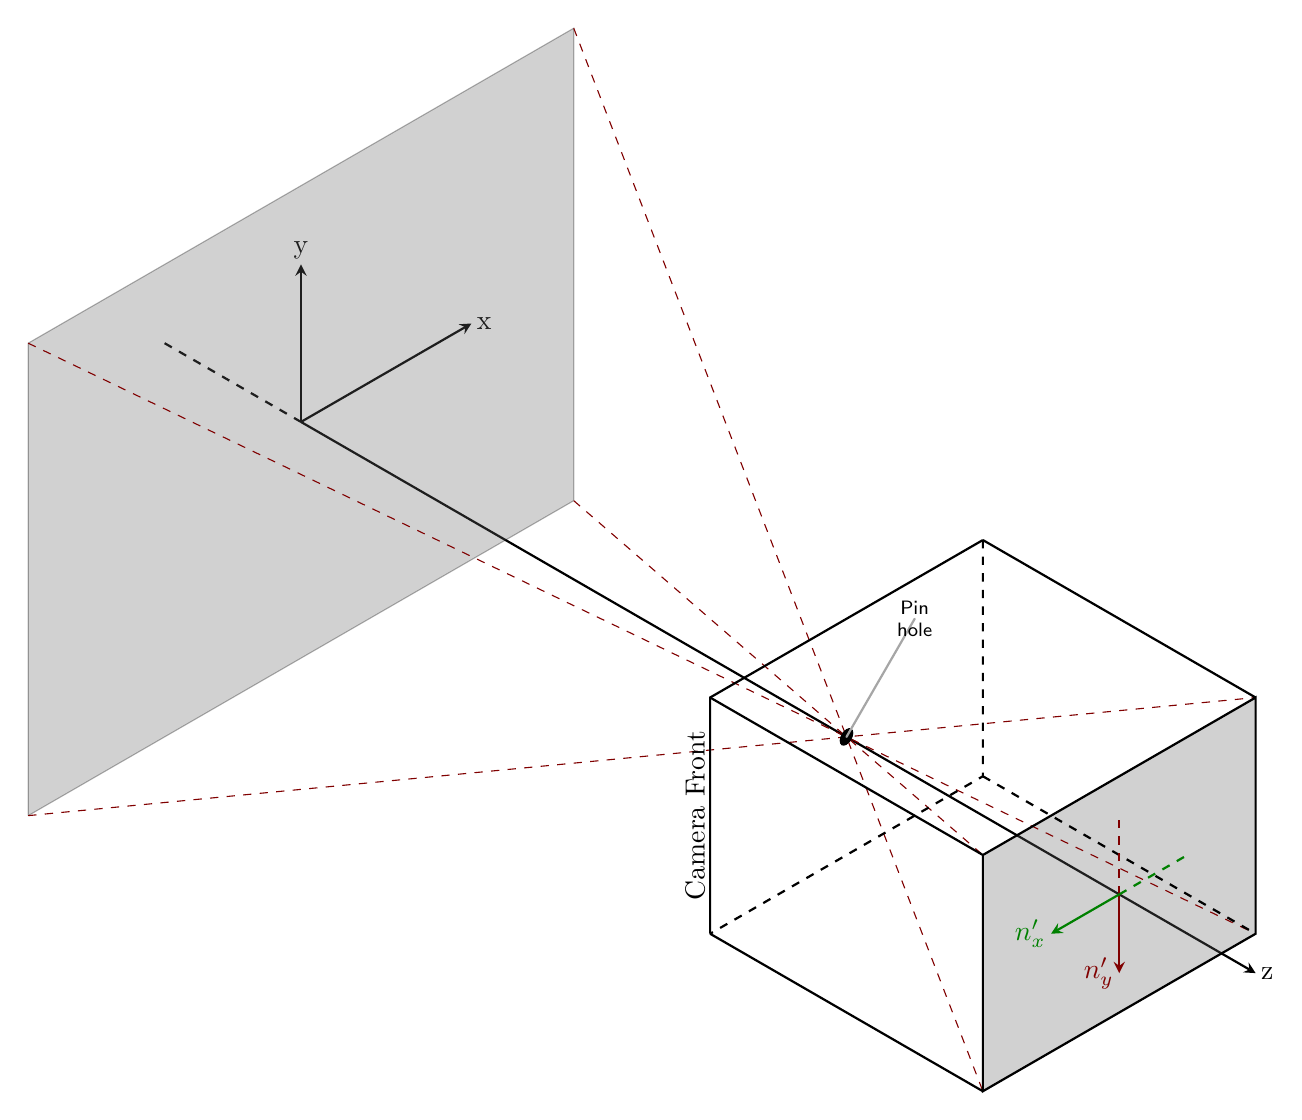
\begin{tikzpicture}[x={(0.866cm,-0.5cm)}, y={(0.866cm,0.5cm)}, z={(0cm,1cm)}, scale=1.0,
    %Option for nice arrows
    >=stealth, %
    inner sep=0pt, outer sep=2pt,%
    axis/.style={thick,->},
    wave/.style={thick,color=#1,smooth},
    polaroid/.style={fill=black!60!white, opacity=0.3},
]
    % Colors
    \colorlet{darkgreen}{green!50!black}
    \colorlet{lightgreen}{green!80!black}
    \colorlet{darkred}{red!50!black}
    \colorlet{lightred}{red!80!black}

    % Frame
    \coordinate (O) at (0, 0, 0);
	\draw[axis] (O) -- +(14, 0,   0) node [right] {z};
    \draw[axis] (O) -- +(0,  2.5, 0) node [right] {x};
    \draw[axis] (O) -- +(0,  0,   2) node [above] {y};

    \draw[thick,dashed] (-2,0,0) -- (O);

    % monochromatic incident light with electric field
   % \draw[wave=blue, opacity=0.7, variable=\x, samples at={-2,-1.75,...,0}]
    %    plot (\x, { cos(1.0*\x r)*sin(2.0*\x r)}, { sin(1.0*\x r)*sin(2.0*\x r)})
    %    plot (\x, {-cos(1.0*\x r)*sin(2.0*\x r)}, {-sin(1.0*\x r)*sin(2.0*\x r)});



    \filldraw[polaroid] (0,-4,-3) -- (0,-4,3) -- (0,4,3) -- (0,4,-3) -- (0,-4,-3);
	
	\filldraw[polaroid] (12,-2,-1.5) -- (12,-2,1.5) -- (12,2,1.5) -- (12,2,-1.5) -- (12,-2,-1.5);
	%\draw[polaroid]   (10, -2,  -1.5) -- (10, -2,   1.5) -- (10, 2, 1.5) -- (10, 2, -1.5) -- cycle;
	\draw[darkred, dashed]   (0, -4, -3) -- (12,2, 1.5);
	\draw[darkred, dashed]   (0, 4, -3) -- (12,-2, 1.5);
	\draw[darkred, dashed]   (0, -4, 3) -- (12,2, -1.5);
	\draw[darkred, dashed]   (0, 4, 3) -- (12,-2, -1.5);

    % Electric field vectors
   % \draw[wave=blue, variable=\x,samples at={0,0.25,...,6}]
    %    plot (\x,{sin(2*\x r)},0)node[anchor=north]{$\vec{E}$};

    %Polarized light between polaroid and thin section
   % \foreach \x in{0, 0.25,...,6}
     %   \draw[color=blue,->] (\x,0,0) -- (\x,{sin(2*\x r)},0);

    %\draw (3,1,1) node [text width=2.5cm, text centered]{Polarized light};

    %Crystal thin section
    \begin{scope}[thick]
        \draw (8,-2,-1.5) -- (8,-2,1.5) node [above, sloped, midway]{Camera Front}--(8, 2, 1.5);
        \draw[dashed] (8, 2, 1.5) -- (8, 2, -1.5)--(8,-2,-1.5)
        (8,   2, -1.5) -- (12,  2,-1.5); % First face
        \draw (8,  -2, -1.5) -- (12, -2,-1.5)
            
            (8,   2,  1.5) -- (12,  2, 1.5)
            (8,  -2,  1.5) -- (12, -2, 1.5)
            (12,-2, -1.5) -- (12, -2, 1.5) -- (12, 2, 1.5) 
                -- (12, 2, -1.5) -- cycle; % Second face

        %Optical indices
        \draw[darkred, ->]       (12, 0, 0) -- (12, 0,  -1) node [left] {$n_{y}'$}; % index 1
        \draw[darkred, dashed]   (12, 0, 0) -- (12,0, 1); % index 1
        \draw[darkgreen, ->]     (12, 0, 0) -- (12, -1,0) node [left] {$n_{x}'$}; % index 2
        \draw[darkgreen, dashed] (12, 0, 0) -- (12,1, 0); % index 2
    \end{scope}

 \begin{scope}[canvas is zy plane at x=8]
%\shade[draw] (-1,-1) rectangle (1,1);
\fill (0,0) circle[radius=0.1cm] ;

\path [draw=gray!70, thick, line cap=round, every node/.style={align=center, font=\scriptsize\sffamily}] (0,0,0) to (1,1,0) node {Pin\\hole};

\end{scope}

	

    %\draw[thick, <->] (12, -1.5,-0.5) -- (12, -1.5, 0.5); %Polarization direction


\end{tikzpicture}
\end{document}